\subsection{Exercise~1.1}

Let more generally~$X$ be any finite set.
We will construct one-to-one correspondences between the following concepts:
\begin{itemize*}

	\item
		A topology on~$X$.

	\item
		A preorder on~$X$.

	\item
		An equivalence relation~$∼$ on~$X$ and a partial order on~$X / {∼}$.

\end{itemize*}

This allows us to list all topologies on finite sets with~$n$ elements for small values on~$n$; namely~$n = 0, 1, 2, 3$.
We can then draw of diagram to see how these topologies are contained in one another.



\subsubsection{First Correspondence: From Topologies to Preorders}

Let~$\top{T}$ be a topology on~$X$.
For every point~$x$ in~$X$ we can consider the set~$\top{T}_x$ of open neighbourhoods of~$x$, i.e.,
\[
	\top{T}_x ≔ \{ V ∈ \top{T} \suchthat x ∈ V \}
\]
We define a preorder~$≤$ on~$X$ via
\[
	x ≤ y \iff \top{T}_x ⊆ \top{T}_y \,.
\]
In other words, we have~$x ≤ y$ if and only if every open neighbourhood of~$x$ is also an open neighbourhood of~$y$.

We can consider for every point~$x$ in~$X$ the intersection~$U x ≔ ⋂ \top{T}_x$.
This intersection is finite, because~$X$ is finite, whence~$U x$ is again contained in~$\top{T}$.
By construction,~$U x$ is the smallest subset of~$\top{T}$ containing~$X$.
Consequently, we have~$x ≤ y$ if and only if~$y ∈ U x$.
The set~$U x$ can therefore be described as
\[
	U x = \{ y ∈ X \suchthat y ≥ x \} \,.
\]

A subset~$V$ of~$X$ contained in~$\top{T}$ if and only if~$V = ⋃_{x ∈ X} U x$.
The open sets~$U x$ with~$x ∈ x$ are therefore a basis for the topology~$\top{T}$.

This entails that the topology~$\top{T}$ can be retrieves from the preorder~$≤$, since it can be retrieved from the assignment~$U$, which in turn is characterized purely in terms of~$≤$.



\subsubsection{First Correspondence: From Preorders to Topologies}

Suppose conversely that~$≤$ is any preorder on~$X$.
For every point~$x$ in~$X$ let~$U x ≔ \{ y ∈ X \suchthat y ≥ x \}$ be the upper set above~$x$.

These sets form a basis for a topology~$\top{T}$ on~$X$:
For every point~$x$ in~$X$ we have~$x ∈ U x$, and thus altogether~$X = ⋃_{x ∈ X} U x$.
For every point~$z$ in~$U x ∩ U y$ we have~$U z ⊆ U x ∩ U y$ by the transitivity of~$≤$.

The subsets of~$X$ contained in~$\top{T}$ are precisely the unions of sets of the form~$U x$ with~$x ∈ X$.
Once again,~$N x$ turns out to be the smallest open set containing~$x$.
To see this, let~$V$ be some set contained in~$\top{T}$ with~$x ∈ V$.
Then there exists some~$y ∈ X$ with~$x ∈ U y ⊆ V$.
We find from~$x ∈ U y$ that~$x ≥ y$ and therefore~$U x ⊆ U y ⊆ V$.

For every two points~$x$ and~$y$ in~$X$ we have therefore the equivalences
\[
	\text{every~$V ∈ \top{T}$ that contains~$x$ also contains~$y$}
	\iff
	y ∈ U x
	\iff
	x ≤ y \,.
\]



\subsubsection{First Correspondence}

The above two constructions between topologies on~$X$ and preorders on~$X$ are mutually inverse.
We have therefore constructed a one-to-one correspondence between topologies on~$X$ and preorders on~$X$.

To construct the topology corresponding to a given preorder~$≤$ we first determine the upper sets~$U x = \{ y ∈ X \suchthat y ≥ x \}$ for every~$x ∈ X$.
We then form all unions of these sets.



\subsubsection{Second Correspondence}

Let~$≤$ be a preorder on~$X$.
We can define an equivalence relation~$∼$ on~$X$ via
\[
	x ∼ y \iff \text{both~$x ≤ y$ and~$y ≤ x$} \,.
\]
The preorder~$≤$ descends to a partial order on the quotient set~$X / {∼}$, given by
\[
	\class{x} ≤ \class{y} \iff x ≤ y \,.
\]

Suppose conversely that~$∼$ is some equivalence relation on~$X$ and that~$≤$ is a partial order on~$X / {∼}$.
We can pull back the partial order~$≤$ along the canonical quotient map from~$X$ to~$X / {∼}$ to a preorder~$≤$ on~$X$ via~$x ≤ y$ if and only if~$\class{x} ≤ \class{y}$.



\subsubsection{Topologies on the Empty Set}

Let~$X = ∅$.
There exists precisely one equivalence relation~$∼$ on the set~$X$, and precisely one partial order on the quotient~$X / {∼} = ∅$.
There hence exists precisely one topology on~$X$, which is given by~$\{ ∅ \}$.



\subsubsection{Topologies on the One-Element Set}

Let~$X = \{ a \}$.
There exists precisely one equivalence relation~$∼$ on the set~$X$, and precisely one partial order on the quotient~$X / {∼} = \{ \{ a \} \}$.
There hence exists precisely one topology on~$X$, which is given by~$\{ ∅, X \}$.


\subsubsection{Topologies on the Two-Element Set}

Let~$X = \{ a, b \}$ be a set with two elements.
There exist two equivalence relations on~$X$.
\begin{itemize}

	\item
		The equivalence relation~$∼$ for which~$a$ and~$b$ are not equivalent.
		There are three partial orders on the quotient set~$X / {∼} = \{ \class{a}, \class{b} \}$.
		\begin{itemize}

			\item
				The elements $\class{a}$ and~$\class{b}$ are not comparable.
				The corresponding preorder on~$X$ is given by having~$a$ and~$b$ be not comparable.
				Then~$U a = \{a\}$ and~$U b = \{b\}$.
				The corresponding topology is given by~$\{ ∅, \{a\}, \{b\}, X \}$.

			\item
				We have $\class{a} ≤ \class{b}$.
				The corresponding preorder on~$X$ is given by~$a ≤ b$.
				Then~$U a = X$ and~$U b = \{ b \}$.
				The corresponding topology on~$X$ is given by~$\{ ∅, \{ b \}, X \}$.

			\item
				We have $\class{b} ≤ \class{a}$.
				The corresponding preorder on~$X$ is given by~$b ≤ a$.
				Then~$U a = \{ a \}$ and~$U b = X$.
				The corresponding topology on~$X$ is given by~$\{ ∅, \{ a \}, X \}$.

		\end{itemize}

	\item
		The equivalence relation~$∼$ with~$a ∼ b$.
		There exists precisely one partial order on the one-element quotient set~$X / {∼}$.
		The corresponding preorder on~$X$ is given by~$a ≤ b$ and~$b ≤ a$.
		Then~$U a, U b = X$.
		The corresponding topology on~$X$ is given by~$\{ ∅, X \}$.

\end{itemize}
We have thus found four topologies on~$X$.



\subsubsection{Topologies on the Three-Element Set}

Let~$X = \{ a, b, c \}$ be a set with three elements.
There exist five equivalence relations on~$X$.

\begin{itemize*}

	\item
		The equivalence relation~$∼$ for which all three elements of~$X$ are non-equivalent.
		On the three-element quotient set~$X / {∼} = \{ \class{a}, \class{b}, \class{c} \}$ we have five types of partial orders, corresponding to the following Hasse diagrams:
		\[
			\centerbox{
			
\begin{tikzpicture}[scale=0.6]
				\draw[fill] (0, 0) circle (0.1);
				\draw[fill] (1, 0) circle (0.1);
				\draw[fill] (2, 0) circle (0.1);
			\end{tikzpicture}
			}
			\hspace{3.5em}
			\centerbox{
			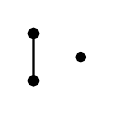
\begin{tikzpicture}[scale=0.6]
				\draw[fill, thick] (0, 0) circle (0.1) -- (0, 1) circle (0.1);
				\draw[fill] (1, 0.5) circle (0.1);
			\end{tikzpicture}
			}
			\hspace{3.5em}
			\centerbox{
			
\begin{tikzpicture}[scale=0.6]
				\draw[fill, thick] (-0.6, 1) circle (0.1) -- (0, 0) circle (0.1) -- (0.6, 1) circle (0.1);
			\end{tikzpicture}
			}
			\hspace{3.5em}
			\centerbox{
			
\begin{tikzpicture}[scale=0.6]
				\draw[fill, thick] (-0.6, 0) circle (0.1) -- (0, 1) circle (0.1) -- (0.6, 0) circle (0.1);
			\end{tikzpicture}
			}
			\hspace{3.5em}
			\centerbox{
			
\begin{tikzpicture}[scale=0.6]
				\draw[fill, thick] (0, 0) circle (0.1) -- (0, 1) circle (0.1) -- (0, 2) circle (0.1);
			\end{tikzpicture}
			}
		\]
		Let us go through these different types of partial orders:
		\begin{description}

			\item[First type]
				All three elements are non-comparable.
				Then
				\[
					U a = \{ a \} \,, \quad
					U b = \{ b \} \,, \quad
					U c = \{ c \} \,.
				\]
				The resulting topology is the discrete topology
				\[
					\top{T}_{29} ≔ \{ ∅, \{a\}, \{b\}, \{c\}, \{a,b\}, \{a,c\}, \{b,c\}, X \} \,.
				\]

			\item[Second type]
				Precisely two elements of~$X / {∼}$ are comparable.

				Suppose first that~$\class{a} ≤ \class{b}$ and that~$\class{c}$ is not comparable to either~$\class{a}$ and~$\class{b}$.
				Then~$U a = \{ a, b \}$,~$U b = \{ b \}$,~$U c = \{ c \}$.
				The resulting topology is
				\[
					\top{T}_{27} ≔
					\{
						∅, \{ b \}, \{ c \}, \{ a, b \}, \{ b, c \}, X
					\} \,.
				\]

				By permuting the roles of~$a$,~$b$ and~$c$, we also get the topologies
				\begin{align*}
					% swap a and b
					\top{T}_{25} &≔ \{ ∅, \{ a \}, \{ c \}, \{ a, b \}, \{ a, c \}, X \} \,,
					\\
					% swap a and b
					\top{T}_{24} &≔ \{ ∅, \{ a \}, \{ b \}, \{ a, b \}, \{ b, c \}, X \} \,,
					\\
					% swap b and c
					\top{T}_{28} &≔ \{ ∅, \{ b \}, \{ c \}, \{ a, c \}, \{ b, c \}, X \} \,,
					\\
					% swap a → b → c
					\top{T}_{26} &≔ \{ ∅, \{ a \}, \{ c \}, \{ a, c \}, \{ b, c \}, X \} \,,
					\\
					% swap c → b → a
					\top{T}_{23} &≔ \{ ∅, \{ a \}, \{ b \}, \{ a, b \}, \{ a, c \}, X \} \,.
				\end{align*}

			\item[Third type]
				All elements of~$X / {∼}$ are comparable, but not linearly comparable, with a least element.

				Suppose first that~$\class{a} ≤ \class{b}, \class{c}$.
				Then~$U a = X$,~$U b = \{ b \}$,~$U c = \{ c \}$.
				The corresponding topology is
				\[
					\top{T}_{19} ≔ \{ ∅, \{ b \}, \{ c \}, \{ b, c \}, X  \} \,.
				\]

				By swapping around the roles of~$a$,~$b$ and~$c$, we also get the topologies
				\[
					\top{T}_{17} ≔ \{ ∅, \{ a \}, \{ b \}, \{ a, b \}, X  \} \,, \quad
					\top{T}_{18} ≔ \{ ∅, \{ a \}, \{ c \}, \{ a, c \}, X  \} \,.
				\]

			\item[Fourth type]
				All elements of~$X / {∼}$ are comparable, but not linearly comparable, with a greatest element.

				Suppose first that~$\class{a}, \class{b} ≤ \class{c}$.
				Then~$U a = \{ a, c \}$,~$U b = \{ b, c \}$,~$U c = \{ c \}$.
				The corresponding topology is
				\[
					\top{T}_{22} ≔ \{ ∅, \{ c \}, \{ a, c \}, \{ b, c \}, X \} \,.
				\]

				By swapping around the roles of~$a$,~$b$ and~$c$, we also get the topologies
				\[
					\top{T}_{20} ≔ \{ ∅, \{ a \}, \{ a, b \}, \{ a, c \}, X \} \,, \quad
					\top{T}_{21} ≔ \{ ∅, \{ b \}, \{ a, b \}, \{ b, c \}, X \} \,.
				\]

			\item[Fifth type]
				All elements of~$X / {∼}$ are linearly comparable.

				Suppose first that~$\class{c} ≤ \class{b} ≤ \class{a}$.
				Then~$U a = \{ a \}$,~$U b = \{ a, b \}$,~$U c = X$.
				The resulting topology is
				\[
					\top{T}_8 ≔ \{ ∅, \{ a \}, \{ a, b \}, X \} \,.
				\]

				By permuting the roles of~$a$,$~b$,~$c$, we get also the topologies
				\begin{align*}
					\top{T}_9    &≔ \{ ∅, \{ a \}, \{ a, c \}, X \} \,, \\
					\top{T}_{11} &≔ \{ ∅, \{ b \}, \{ a, b \}, X \} \,, \\
					\top{T}_{13} &≔ \{ ∅, \{ b \}, \{ b, c \}, X \} \,, \\
					\top{T}_{15} &≔ \{ ∅, \{ c \}, \{ a, c \}, X \} \,, \\
					\top{T}_{16} &≔ \{ ∅, \{ c \}, \{ b, c \}, X \} \,.
				\end{align*}

		\end{description}

	\item
		The elements~$b$ and~$c$ are equivalent, but not equivalent to~$a$.
		On the two-element quotient set~$X / {∼} = \{ \{ a \}, \{ b, c \} \}$ we have three partial orders.
		\begin{description}

			\item[First type]
				The elements of~$X / {∼}$ are not comparable.
				Then
				\[
					U a = \{ a \} \,, \quad
					U b, U c = \{ b, c \} \,.
				\]
				The resulting topology is
				\[
					\top{T}_{10} ≔ \{ ∅, \{ a \}, \{ b, c \}, X \} \,.
				\]

			\item[Second type]
				We have~$\{ a \} ≤ \{ b, c \}$.
				Then~$U a = X$ and~$U b, U c = \{ b, c \}$.
				The resulting topology is
				\[
					\top{T}_7 ≔ \{ ∅, \{ b, c \}, X \} \,.
				\]

			\item[Third type]
				We have~$\{ b, c \} ≤ \{ a \}$.
				Then~$U a = \{ a \}$ and~$U b, U c = X$.
				The resulting topology is
				\[
					\top{T}_2 ≔ \{ ∅, \{ a \}, X \}
				\]

		\end{description}

		By swapping the roles the~$a$,~$b$ and~$c$ around, we get the following additional topologies:
		\begin{gather*}
			% all permutations of { ∅, {a}, {b, c}, X }
			\top{T}_{12} ≔ \{ ∅, \{ b \}, \{ a, c \}, X \} \,, \quad
			\top{T}_{14} ≔ \{ ∅, \{ c \}, \{ a, b \}, X \} \,, \quad
			% all permutations of { ∅, {b, c}, X }
			\top{T}_5 ≔ \{ ∅, \{ a, b \}, X \} \,,
			\\
			\top{T}_6 ≔ \{ ∅, \{ a, c \}, X \} \,, \quad
			% permutations of \{ ∅, \{ a \}, X \}
			\top{T}_3 ≔ \{ ∅, \{ b \}, X \} \,, \quad
			\top{T}_4 ≔ \{ ∅, \{ c \}, X \} \,.
		\end{gather*}

	\item
		All three elements of~$X$ are equivalent.
		The quotient set~$X / {∼}$ consists of one element, whence there is precisely one partial order on it.
		The corresponding topology is given by the indiscrete topology
		\[
			\top{T}_1 ≔ \{ ∅, X \} \,.
		\]

\end{itemize*}

We have overall found~$29$ topologies on the three-element set~$X = \{ a, b, c \}$.
The inclusions between these topologies is depicted in \cref{topologies on a three element set}.
\begin{figure}
	\centering
	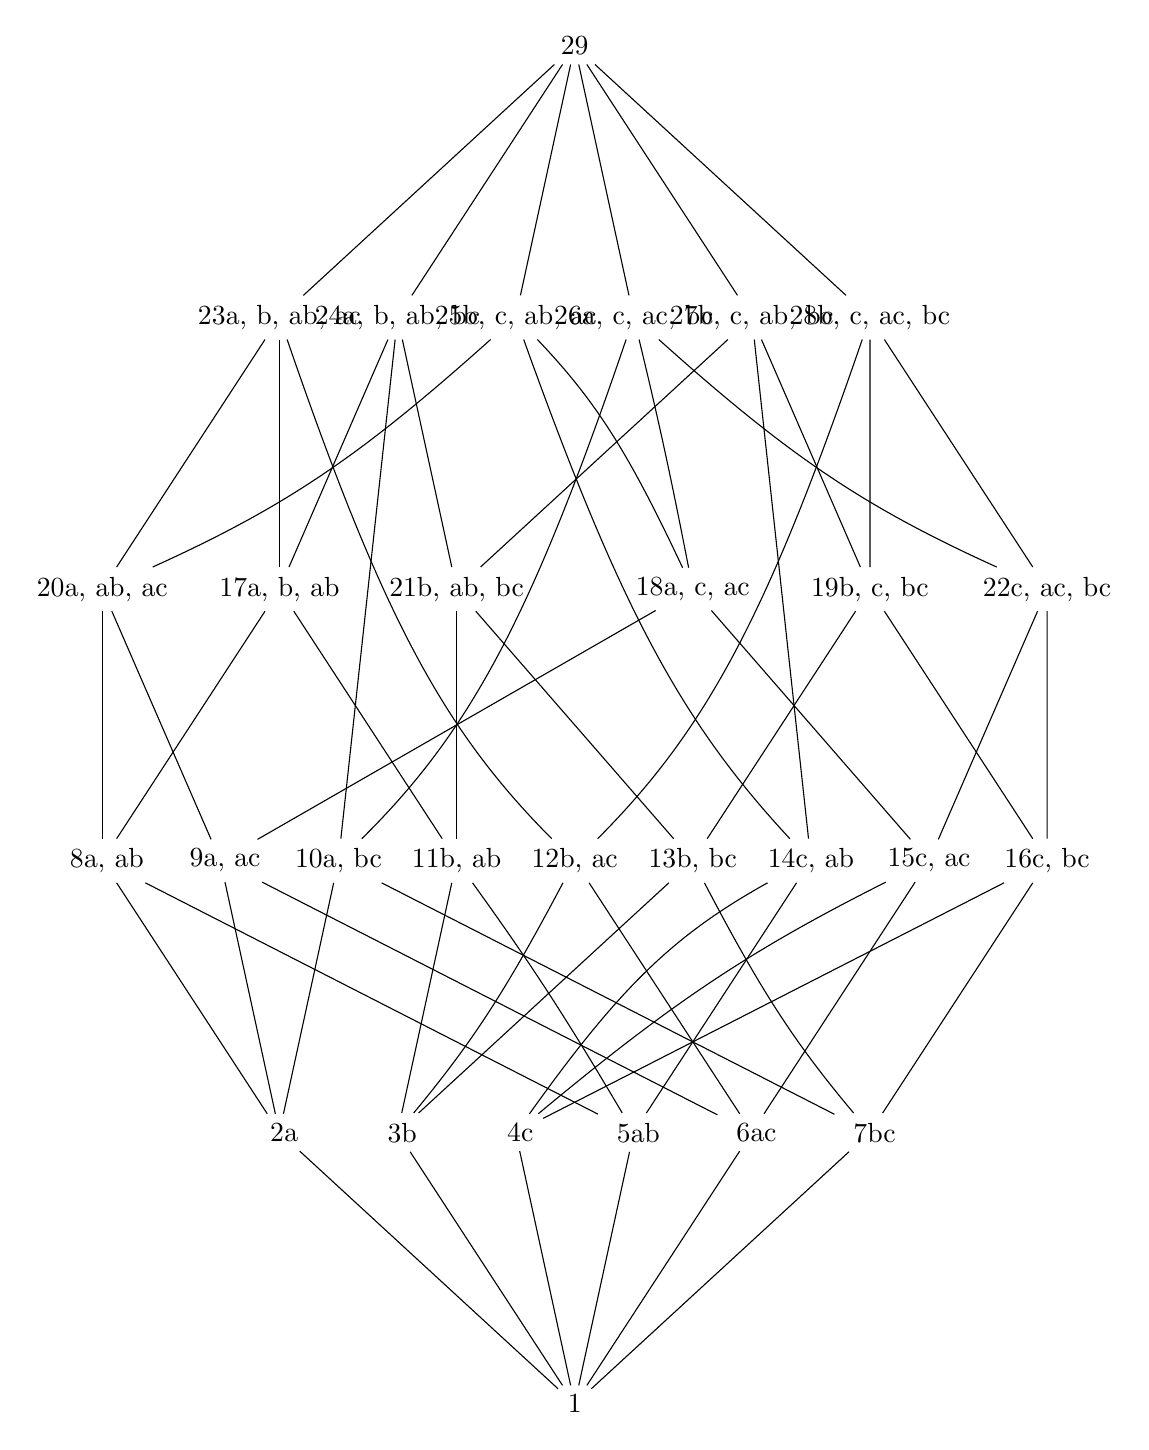
\begin{tikzpicture}[xscale = 0.75, yscale = 3.45]
		% no elements
		\node  (1) at ( 8, 0) {$1$};
		% one element
		\node  (2) at ( 3, 1) {\topel{ 2}{a}};
		\node  (3) at ( 5, 1) {\topel{ 3}{b}};
		\node  (4) at ( 7, 1) {\topel{ 4}{c}};
		\node  (5) at ( 9, 1) {\topel{ 5}{ab}};
		\node  (6) at (11, 1) {\topel{ 6}{ac}};
		\node  (7) at (13, 1) {\topel{ 7}{bc}};
		% two elements
		\node  (8) at ( 0, 2) {\topel{ 8}{a, ab}};
		\node  (9) at ( 2, 2) {\topel{ 9}{a, ac}};
		\node (10) at ( 4, 2) {\topel{10}{a, bc}};
		\node (11) at ( 6, 2) {\topel{11}{b, ab}};
		\node (12) at ( 8, 2) {\topel{12}{b, ac}};
		\node (13) at (10, 2) {\topel{13}{b, bc}};
		\node (14) at (12, 2) {\topel{14}{c, ab}};
		\node (15) at (14, 2) {\topel{15}{c, ac}};
		\node (16) at (16, 2) {\topel{16}{c, bc}};
		% three elements
		\node (20) at ( 0, 3) {\topel{20}{a, ab, ac}};
		\node (17) at ( 3, 3) {\topel{17}{a, b, ab}};
		\node (21) at ( 6, 3) {\topel{21}{b, ab, bc}};
		\node (18) at (10, 3) {\topel{18}{a, c, ac}};
		\node (19) at (13, 3) {\topel{19}{b, c, bc}};
		\node (22) at (16, 3) {\topel{22}{c, ac, bc}};
		% four elements
		\node (23) at ( 3, 4) {\topel{23}{a, b, ab, ac}};
		\node (24) at ( 5, 4) {\topel{24}{a, b, ab, bc}};
		\node (25) at ( 7, 4) {\topel{25}{b, c, ab, ac}};
		\node (26) at ( 9, 4) {\topel{26}{a, c, ac, bc}};
		\node (27) at (11, 4) {\topel{27}{b, c, ab, bc}};
		\node (28) at (13, 4) {\topel{28}{b, c, ac, bc}};
		% six elements
		\node (29) at ( 8, 5) {$29$};
		% arrows from no elements to one element;
		\draw  (1) --  (2);
		\draw  (1) --  (3);
		\draw  (1) --  (4);
		\draw  (1) --  (5);
		\draw  (1) --  (6);
		\draw  (1) --  (7);
		% arrows from one elements to two elements
		\draw  (2) --  (8);
		\draw  (2) --  (9);
		\draw  (2) -- (10);
		\draw  (3) -- (11);
		\draw  (3) to[bend right = 3.8] (12);
		\draw  (3) -- (13);
		\draw  (4) to[bend left  = 5] (14);
		\draw  (4) to[bend left  = 2] (15);
		\draw  (4) -- (16);
		\draw  (5) --  (8);
		\draw  (5) to[bend right = 1.7] (11);
		\draw  (5) -- (14);
		\draw  (6) --  (9);
		\draw  (6) -- (12);
		\draw  (6) -- (15);
		\draw  (7) -- (10);
		\draw  (7) to[bend left  = 4] (13);
		\draw  (7) -- (16);
		% arrows from two elements to three elements
		\draw  (8) -- (17);
		\draw  (8) -- (20);
		\draw  (9) -- (18);
		\draw  (9) -- (20);
		\draw (11) -- (17);
		\draw (11) -- (21);
		\draw (13) -- (19);
		\draw (13) -- (21);
		\draw (15) -- (18);
		\draw (15) -- (22);
		\draw (16) -- (19);
		\draw (16) -- (22);
		% arrows from two elements to four elements
		\draw (10) -- (24);
		\draw (10) to[bend right = 10.2] (26);
		\draw (12) to[bend left  = 10] (23);
		\draw (12) to[bend right = 10] (28);
		\draw (14) to[bend left  = 9] (25);
		\draw (14) -- (27);
		% arrows from three elements to four elements
		\draw (17) -- (23);
		\draw (17) -- (24);
		\draw (18) to[bend right = 6] (25);
		\draw (18) to[bend right = 3] (26);
		\draw (19) -- (27);
		\draw (19) -- (28);
		\draw (20) -- (23);
		\draw (20) to[bend right = 2.7] (25);
		\draw (21) -- (24);
		\draw (21) -- (27);
		\draw (22) to[bend left  = 2.7] (26);
		\draw (22) -- (28);
		% arrows from four elements to six elements
		\draw (23) -- (29);
		\draw (24) -- (29);
		\draw (25) -- (29);
		\draw (26) -- (29);
		\draw (27) -- (29);
		\draw (28) -- (29);
	\end{tikzpicture}
	\caption{The topologies on~$\{ a, b, c \}$.}
	\label{topologies on a three element set}
\end{figure}
